% To do:
% Wei: Recurrent layer is concatnateded or added with the previous layers?. (add)
% Do we need to mention the norm?

\section{Model Architecture}

\begin{figure}[htb]
\begin{center}
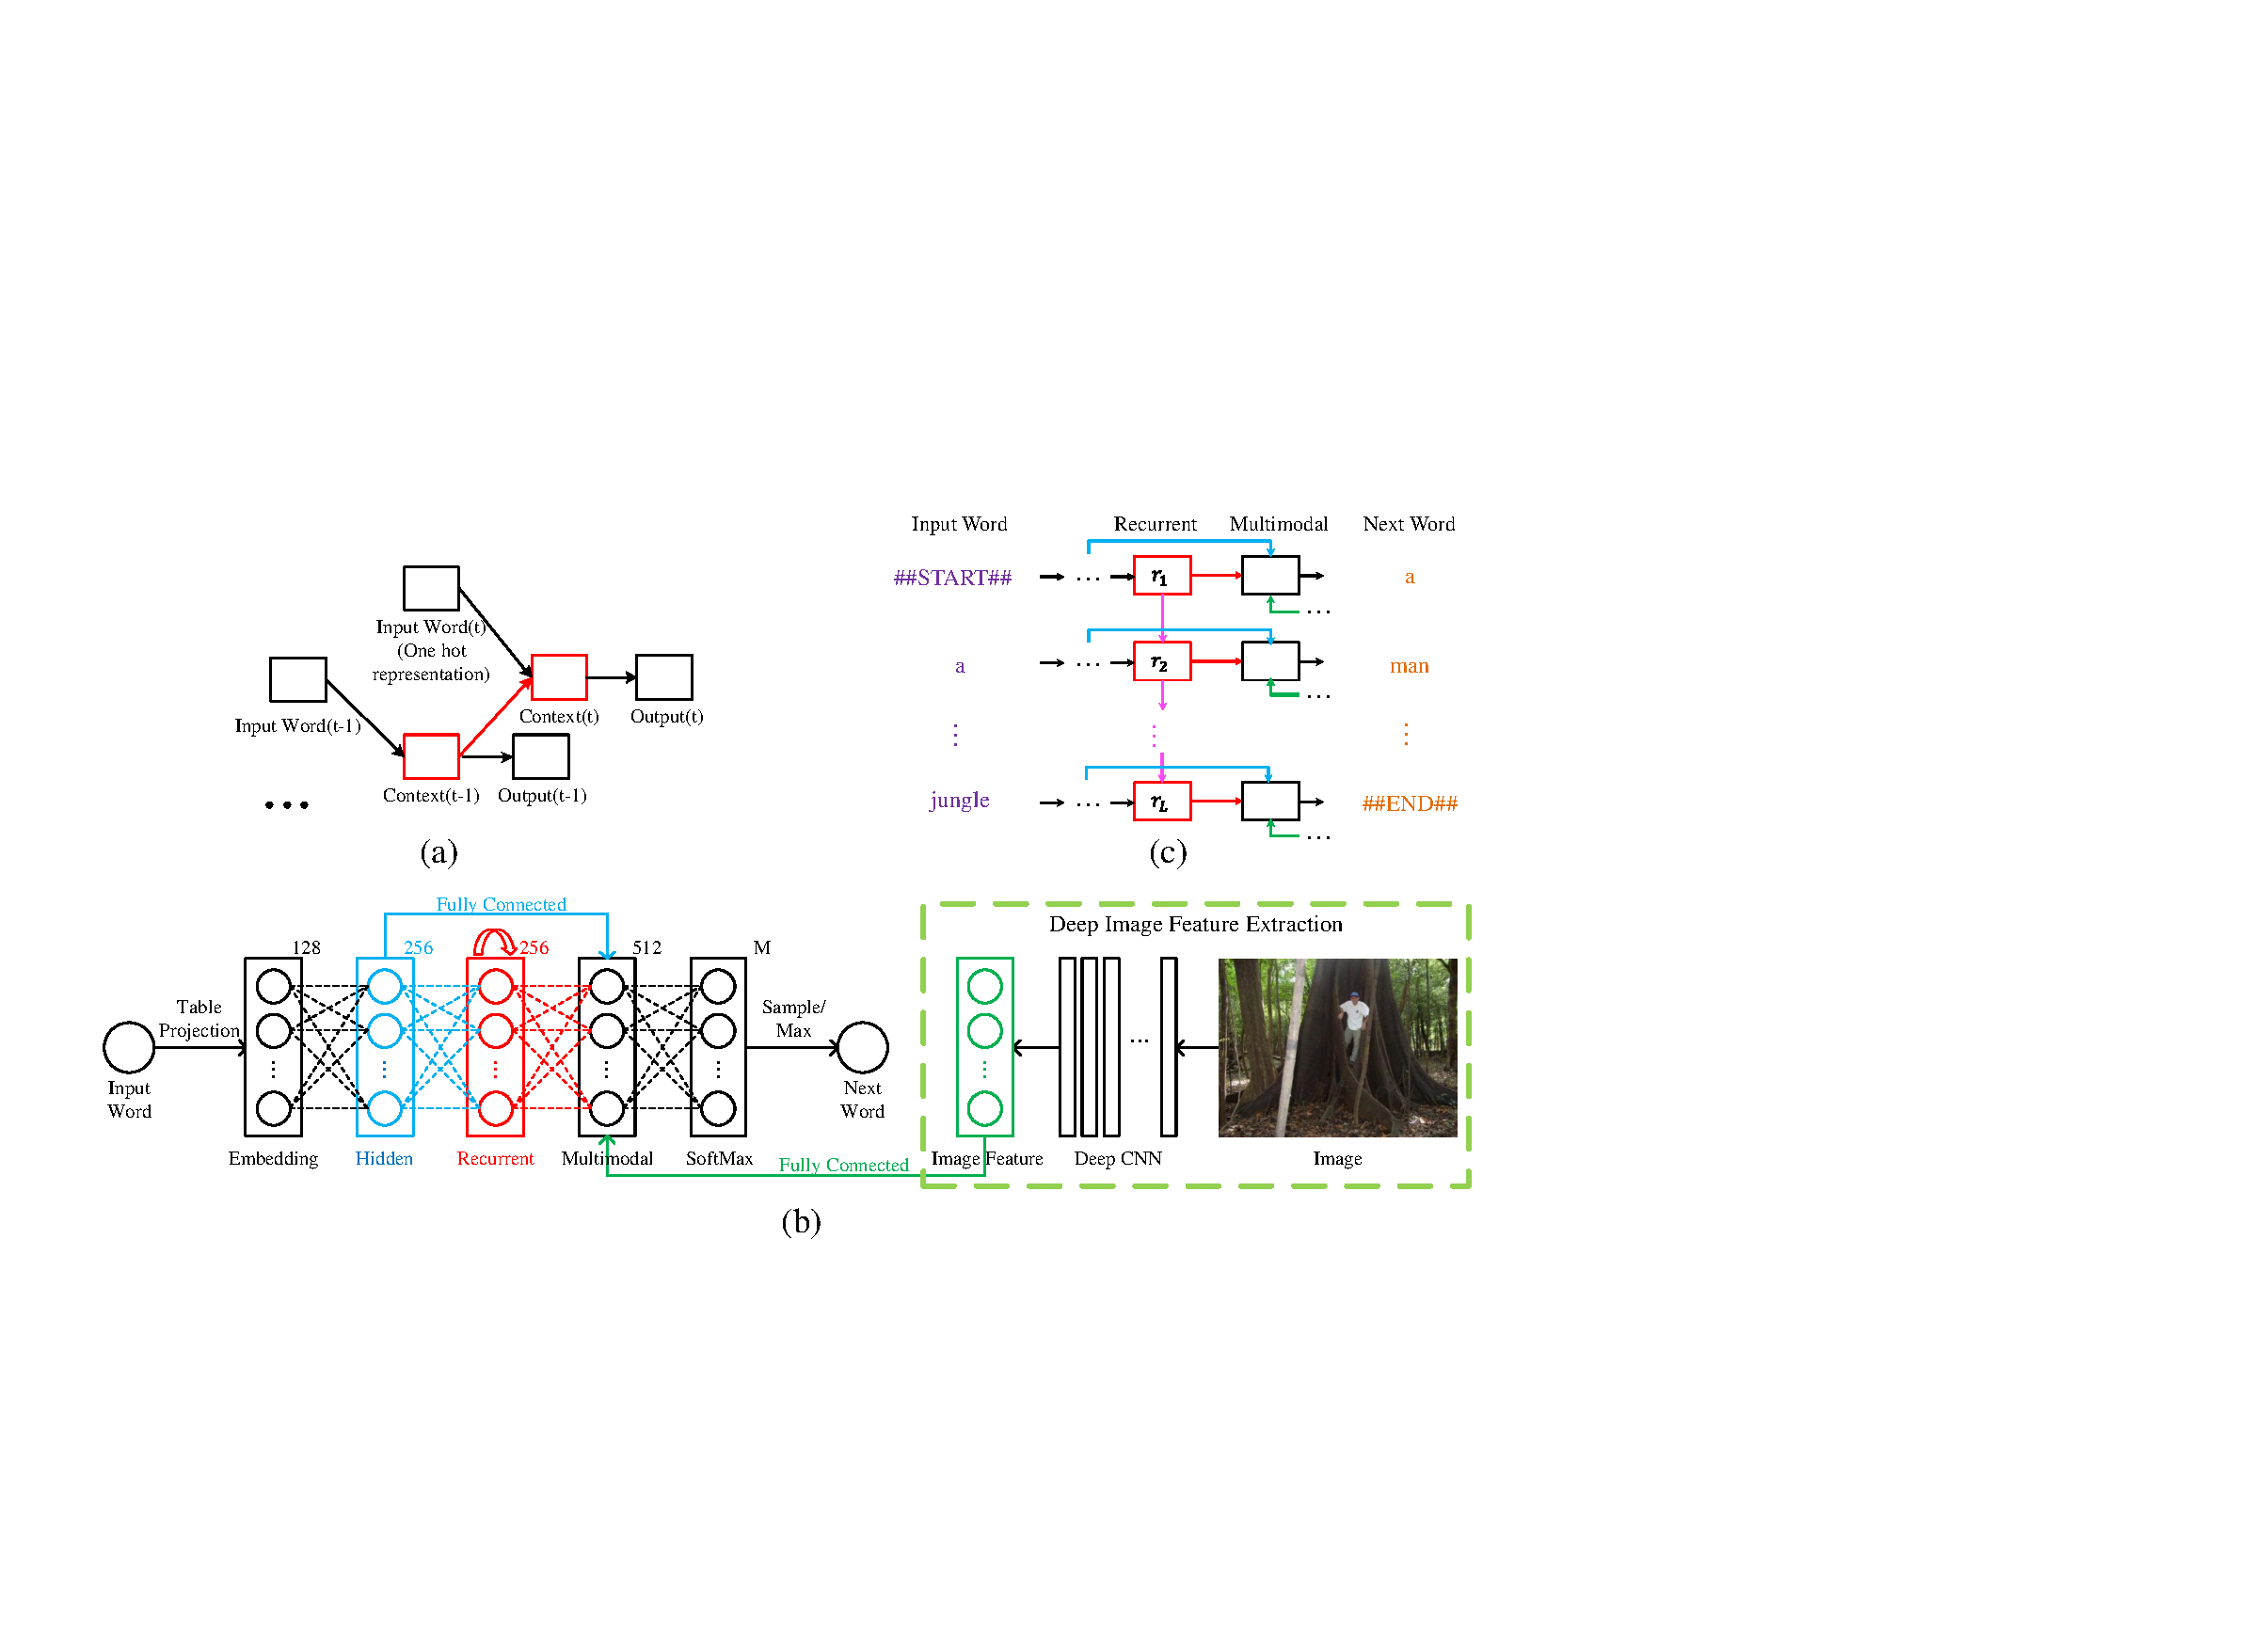
\includegraphics[width=0.95\linewidth]{PaperFigures/arch_final_visio.pdf}
\end{center}
   \caption{Illustration of the basic Recurrent Neural Network (RNN) and our multimodal Recurrent Neural Network (m-RNN) architecture.
   (a). The basic RNN architecture. 
   (b). The architecture of m-RNN model.
   The input of the model is an image and its corresponding sentences. (e.g. the sentence for the shown image is: \emph{a man at a giant tree in the jungle}. 
   The model will estimate the probability distribution of the next word given previous words and the image.
   This architecture is deeper than the basic RNN.
   % of structure without considering the extendibility of the recurrent layer.
   (c). The illustration of how the recurrent layer works in m-RNN. 
   % We can unfold the recurrent layer, which leads to the temporal depth of the network.
   The model parameters are shared for each temporal session of the unfolded m-RNN model.
   }
\label{fig:illu_RNN}
\end{figure}

% For layer \textcircled{\raisebox{-0.9pt}{1}} and layer \textcircled{2},
\subsection{Basic recurrent neural network}
We briefly introduce the basic Recurrent Neural Network (RNN) \cite{elman1990finding,mikolov2010recurrent,mikolov2011extensions} that is widely used for many natural language processing tasks, such as speech recognition.
Its architecture is shown in Figure \ref{fig:illu_RNN}(a).
It has three types of layers in each time session: the input word layer $\mathbf{w}$, the context layer $\mathbf{s}$ and the output layer $\mathbf{y}$.
The activation of input, context and output layers in time $t$ is denoted as $\mathbf{w}(t)$, $\mathbf{s}(t)$, and $\mathbf{y}(t)$.
$\mathbf{w}(t)$ is the one-hot representation of the current word. 
This representation is binary, and has the same dimension of the vocabulary size with only one non-zero element.
$y(t)$ can be calculated as follows:
\begin{equation}
\mathbf{x}(t) = [\mathbf{w}(t)^T\ \ \mathbf{s}(t-1)^T]^T;\ \ \ 
\mathbf{s}(t)=f_1(\mathbf{U} \cdot \mathbf{x}(t));\ \ \ 
\mathbf{y}(t)=g_1(\mathbf{V} \cdot \mathbf{s}(t));
\end{equation}
where $\mathbf{x}(t)$ as a vector that concatenates $\mathbf{w}(t)$ and $\mathbf{s}(t-1)$, $f_1(.)$ and $g_1(.)$ are element-wised sigmoid and softmax function respectively.

We define two types of ``depths'' for a RNN architecture. 
We denote the number of layers in each time session as the \emph{structure depth} (e.g. the structure depth of the basic RNN is 3).
When we compare the depth of different RNN networks, we refer to the structure depth.
The second depth is denoted as the \emph{temporal depth}. 
% Although the structure of the basic RNN model is simple, it is a very deep network which can be unfolded in time sequences.
Accordingly, when we do the backpropagation, we need to propagate the error through recurrent connections back in time \cite{rumelhart1988learning}.

\subsection{Our m-RNN model}
The structure of our multimodal Recurrent Neural Network (m-RNN) is shown in Figure \ref{fig:illu_RNN}(b).
The m-RNN model is much deeper than the basic RNN model.
Its structure depth is 7 (i.e. input word layer, word embedding layer, hidden layer, recurrent layer, multimodal layer, softmax layer and the next word layer).

The word embedding layer learns a initial dense word embedding representation to replace the one-hot representation in basic RNN.
It has several advantages.
Firstly, it will significantly lower the number of parameters in the networks because the dense word vector (128 dimension) is much smaller than the one-hot word vector.
Secondly, the dense word embedding encodes the semantic meanings of the words.
We can find the semantically relevant words by calculating the Euclidean distance between two dense word vectors.

Most of the sentence-image multimodal models \cite{karpathy2014fragment,frome2013devise,socher2014grounded,kiros2013multimodal} use pre-computed word embedding vectors as the initialization of their model. 
In contrast, we randomly initialize our word embedding layers and learn them from the training data.
We show that this random initialization is enough for our architecture to generate the state-of-the-art results.
To further refine the word representation, we add a hidden layer after the initial word embedding layer and treat the activation of the hidden layer as the final word representation.

After the hidden layer, we have a recurrent layer with 256 dimensions.
The calculation of the recurrent layer is slightly different from the basic RNN.
Instead of concatenating the word representation in time $t$ and the recurrent layer vector in time $t-1$, we first map the word representation in time $t$ and context in time $t-1$ into a same vector space and add them together:
\begin{equation}
\mathbf{s}(t)=f_2(\mathbf{U}_w \cdot \mathbf{w}(t) + \mathbf{U}_s \cdot \mathbf{s}(t-1));
\end{equation}
where $\mathbf{s}$ and $\mathbf{w}$ denotes the recurrent layer vector and the word representation respectively.
% This strategy will reduce the number of parameters and accelerate the training and testing process.

Inspired by the recent success of the Rectified Linear Unit (ReLU) in training very deep structure in computer vision field \cite{krizhevsky2012imagenet}, we replace the element-wised sigmoid function in basic RNN with ReLU function.
ReLU is faster, and harder to saturate or overfit the data than many non-linear functions, such as sigmoid.
Previous methods \cite{mikolov2010recurrent,mikolov2011extensions} need to conduct backpropagation through time (BPTT) \cite{rumelhart1988learning} for RNN suffers from the vanishing gradient problem because even the simplest the RNN model has a large temporal depth.
They need to use some heuristics, such as truncated BPTT, to avoid this problem.
Truncated BPTT will stop the BPTT after $k$ time steps, where $k$ is a hand-defined hyperparameter.
Because of the good properties of ReLU, we do not need to stop the BPTT at early stage, which leads to a better and more efficient utilization of the data than truncated BPTT.

After the recurrent layer, we set up a 512 dimensional multimodal layer that connect the language model part and the image part of the whole m-RNN model.
The language model part includes the hidden layer (the word representation) and the recurrent layer (the language context).
The image part contains the image features.
Here we connect the seventh layer of AlexNet \cite{krizhevsky2012imagenet} to the multimodal layer (please refer to Section \ref{sec:ImgSenFeat} for more details).
But our framework can utilize any image features.
We map the feature vector for each layer to a same feature space and add them together to obtain the feature vector for the multimodal layer:
\begin{equation}
\mathbf{m}(t)=g_2(\mathbf{V}_w \cdot \mathbf{w}(t) + \mathbf{V}_s \cdot \mathbf{s}(t) + \mathbf{V}_I \cdot \mathbf{I});
\end{equation}
where $\mathbf{w}$ denotes the multimodal layer feature vector, $\mathbf{I}$ denotes the image feature, $g_2(.)$ is the element-wised scaled hyperbolic tangent function:
\begin{equation}
g_2(x) = 1.7159 \cdot \tanh( \frac{2}{3} x)
\end{equation}
This function will force the gradients into the most non-linear value range and can accelerate the training process than the basic hyperbolic tangent function \cite{lecun2012efficient}.

%We do not restrict the norm the three feature layers that connect to the multimodal layer.
%Our experiments shows that the L2 norm of the hidden layer, 

As the basic RNN, our m-RNN model has a softmax layer that will generate the probability distribution of next word.
The dimension of this layer is the vocabulary size $M$, which is different for different datasets.

\section{Training Objective}
\label{sec:trainCost}
We use the average logarithm of the \emph{Perplexity} of the sentences in the training set given their corresponding images as the cost function of our m-RNN model.
Perplexity is a standard approach to evaluating language model.
The perplexity for one word sequence (i.e. a sentences) $w_{1:L}$ can be calculated as follows, $L$ is the length of the word sequences:
\begin{equation}
\log_2 \mathcal{PPL}(w_{1:L}|\mathbf{I}) = -\frac{1}{L} \sum_{n=1}^{L} \log_2 P(w_n|w_{1:n-1},\mathbf{I})
\end{equation}
where $\mathcal{PPL}(w_{1:L}|\mathbf{I})$ denotes the perplexity of the sentence $w_{1:L}$ given the image $\mathbf{I}$.
$P(w_n|w_{1:n-1},\mathbf{I})$ is the probability of the current word $w_n$ given $\mathbf{I}$ and previous words $w_{1:n-1}$.
It corresponds to the feature vector of the SoftMax layer of our modal.

The cost function of our model is the average of the logarithm of the perplexity for all the sentences in the training set:
\begin{equation}
\mathcal{C} = -\frac{1}{N} \sum_{i=1}^{N} \log_2 \mathcal{PPL}(w_{1:L}^{(i)}|\mathbf{I}^{(i)})
\end{equation}
where $N$ is the number of sentences in the training set.
It is equivalent to the reciprocal of the geometric mean of the probability for the model to generate the training sentences.
Our training objective is to minimize this cost function, which is equivalent to maximize the probability of the model to generate the sentences in the training set given their corresponding images.
The cost function is derivable thus we can use backpropagation to learn the model parameters.

\section{Learning of Image and Sentence Features}
\label{sec:ImgSenFeat}

The architecture of our model allows the gradients from the loss function to be backpropagated to both the language modeling part (i.e. the word embedding, hidden and the recurrent layers) as well as the image part (e.g. the AlexNet \cite{krizhevsky2012imagenet}).

For the language modeling part, as mentioned above, we randomly initialize the language modeling layers and learn their parameters. For the image part, we connect the seventh layer of a pre-trained Convolutional Neural Network \cite{krizhevsky2012imagenet,donahue2013decaf} (aso denoted as AlexNet).
The same features extract from the seventh layer of AlexNet (also denoted as decaf features \cite{donahue2013decaf}) was widely used by previous multimodal methods \cite{kiros2013multimodal,frome2013devise,karpathy2014fragment,socher2014grounded}.
In a most recent work \cite{karpathy2014fragment}, the same image features combined with the state-of-the-art detection framework of Region-CNN \cite{girshick2014rcnn} were used.
Their experiments showed that using this detection framework will indeed increase the performance.
In the experiments, we will show that our method performs much better than \cite{karpathy2014fragment} when the same image features are used, and even better than their results of more sophisticated detection features in terms of many evaluation metrics.

We can update the AlexNet according to the gradient backpropagated from the multimodal layer. In this paper, we fix the image features and the deep CNN network in the training stage due to the luck of the data (The datasets we used in the experiment have less than 30K images).
In the future work, we will try our method on large dataset and finetune the parameters of the deep CNN network in the training stage.

\section{Sentence Generation, Image and Sentence Retrieval}
After training of the m-RNN model, we can use the model for the tasks of sentence generation, image retrieval using sentences and sentence retrieval using images.

The sentence generation process is straight forward.
Start from the start sign ``\#\#START\#\#'' or any length of the context words (e.g. we can give the first words in the reference sentences), our model can calculate the probability distribution of the next word: $P(w|w_{1:n-1},\mathbf{I})$.
Then we can sample from this probability distribution to pick the next word.
In practice, we find that picking the word with the maximum probability will perform slightly better than sampling.
After that, we input the picked word to the model and sample the next word.
This process repeated until we have the end sign ``\#\#END\#\#''.

For the retrieval tasks, we can use our model to calculate the perplexity of generating a sentence given an image.
The perplexity can be treated as an affinity measurement between sentences and images.
For the image retrieval task, we just need to retrieve the images that generate the minimum perplexity with the sentence query. 

The sentence retrieval tasks is trickier because there might be some sentences that has high probability to any image query.
Instead of looking at the perplexity or the probability of the sentences given the query image, we need to use the normalized probability for each sentence: $P(w_{1:L}|\mathbf{I}) / \sum_{\mathbf{I^{'}}} P(w_{1:L}|\mathbf{I^{'}})$ where $\mathbf{I^{'}}$ are images sampled from the training set, $P(w_{1:L}|\mathbf{I}) = \mathcal{PPL}(w_{1:L}|\mathbf{I}) ^ {-L}$.